\chapter{Signal models and simulated samples}
\label{ch:samples}
\epigraph{\emph{“Champions keep playing until they get it right.”}}{Billie Jean King}


Simulation of the different physical processes and the response of the detector to them is necessary to optimise and estimate the performance of the different analyses. In addition, it allows the strategies used in particle identification to be developed prior to the data-taking and the efficiencies of the algorithms to be tested. The preparation of searches for new physics requires a detailed simulation of the detector to estimate its discovery potential and to develop optimal methods for measuring particle properties. A correct understanding of the signal and background processes is essential to distinguish between the two. Once real collision data is available, simulated data is also needed to find deviations from the \ac{SM}. All the steps in the \ac{MC} simulation was described in detail in \Sect{\ref{sec:theory:mc_simulation}}.

Similarly to any physics analysis at the \ac{LHC}, this analysis makes use of simulated samples, both to understand the possible signals to be discovered, and to do a correct modeling of the background with \gammajet final states.
In this chapter, details on the signal and background samples generation and simulation are given.


\section{Signals}
\label{sec:samples:samples:sig}

\subsection{Excited quarks}
\label{subsec:samples:samples:sig:qstar}

One of the two benchmark theories to be tested correspond to \ac{EQ}, which were explained in detail in \Sect{\ref{subsec:theory:bsm:qstar}}. If quarks are composed of more fundamental constituents bound together by some unknown interaction, new effects should appear depending on the value of the compositeness scale \(\Lambda\).
It was also seen that \acp{EQ} couple to the \ac{SM} bosons, whose strengths are determined by the coupling constants \(f\), \(f'\) and \(f_s\).

In this theory, there are a total of 5 parameters: the compositeness scale \(\Lambda\), the three couplings and the \ac{EQ} mass. In order to reduce the number of parameters, it is usual to set \(\Lambda = \mq\)~\cite{Zhan_Li_Liu_Li-2016}, and to take the three coupling constants to be the same. In this way, only the mass and the coupling are the free parameters of the theory.

Samples of \ac{EQ} events are produced using \pythia 8.245~\cite{Pythia8.2} with the \ac{LO} NNPDF 2.3~\cite{NNPDF2} \ac{PDF1} set and the A14 set of tuned parameters for the underlying event.
For the first time at the \ac{LHC} in \gammajet final states, three different flavors are considered: light \acp{EQ} \qstar (\(u^* / d^*\)), and heavy resonances, separating between \cstar and \bstar. Moreover, different couplings are studied in this work, where the following values are used: \(f = 0.01, \, 0.1, \, 0.5, \, 0.75, \, 1.0\). The \ac{EQ} masses and couplings used are listed in \Tab{\ref{tab:samples:samples:sig:qstar:xs}}, where the processes cross-section times branching ratio are shown. Moreover, all the cross-section values are shown in \Fig{\ref{tab:samples:samples:sig:qstar:xs}}.

\begin{table}[ht!]
    \centering
    \caption{Cross-section times branching ratio [fb] of the \ac{EQ} model, for the three considered flavours using different coupling values.}
    \resizebox{\linewidth}{!}{
        \begin{tabular}{lcccccc}
            \toprule
            \multirow{2}{*}{Excited quark}  & \multirow{2}{*}{Mass [GeV]}  
            & \multicolumn{5}{c}{Couplings \(f=f'=f_s\)}
            \\
            \cmidrule(l){3-7}
            &           & 0.01          & 0.10      & 0.50          & 0.75      & 1.00          \\
            \midrule
            \multirow{10}{*}{\(\qstar \rightarrow \gamma + u/d\)}
            & $500$     & 29.9400       & 3007.0000 & 75240.0000    & -         & 304200.0000   \\
            & $1000$    & 1.6560        & 165.0000  & 4153.0000     & -         & 16490.0000    \\
            & $2000$    & 0.0536        & 5.3800    & 133.2000      & -         & 520.8000      \\
            & $3000$    & -             & 0.4435    & 11.0200       & -         & 43.0600       \\
            & $4000$    & -             & 0.0488    & 1.2270        & -         & 4.8240        \\
            & $5000$    & -             & -         & 0.1450        & -         & 0.5877        \\
            & $5500$    & -             & -         & -             & -         & 0.2064        \\
            & $6000$    & -             & -         & 0.0163        & 0.0384    & 0.0719        \\
            & $6500$    & -             & -         & -             & -         & 0.0250        \\
            & $7000$    & -             & -         & -             & 0.0043    & 0.0088        \\
            \midrule
            \multirow{5}{*}{\(\cstar \rightarrow \gamma + c\)}
            & $500$     & 3.6540        & 362.2000  & 9051.0000     & -         & 36290.0000    \\
            & $1000$    & 0.1333        & 13.3400   & 332.4000      & -         & 1297.0000     \\
            & $2000$    & -             & 0.2434    & 6.0190        & -         & 23.6800       \\
            & $3000$    & -             & -         & 0.3135        & -         & 1.2450        \\
            & $4000$    & -             & -         & -             & -         & 0.0906        \\
            \midrule
            \multirow{5}{*}{\(\bstar \rightarrow \gamma + b\)}
            & $500$     & 0.6381        & 63.7700   & 1588.0000     & -         & 6324.0000     \\
            & $1000$    & 0.0220        & 2.2080    & 54.7600       & -         & 215.4000      \\
            & $2000$    & -             & 0.0372    & 0.9249        & -         & 3.6200        \\
            & $3000$    & -             & -         & 0.0446        & -         & 0.1770        \\
            & $4000$    & -             & -         & -             & -         & 0.0121        \\
            \bottomrule
        \end{tabular}
    }
    \label{tab:samples:samples:sig:qstar:xs}
\end{table}

\begin{figure}[ht!]
    \centering
    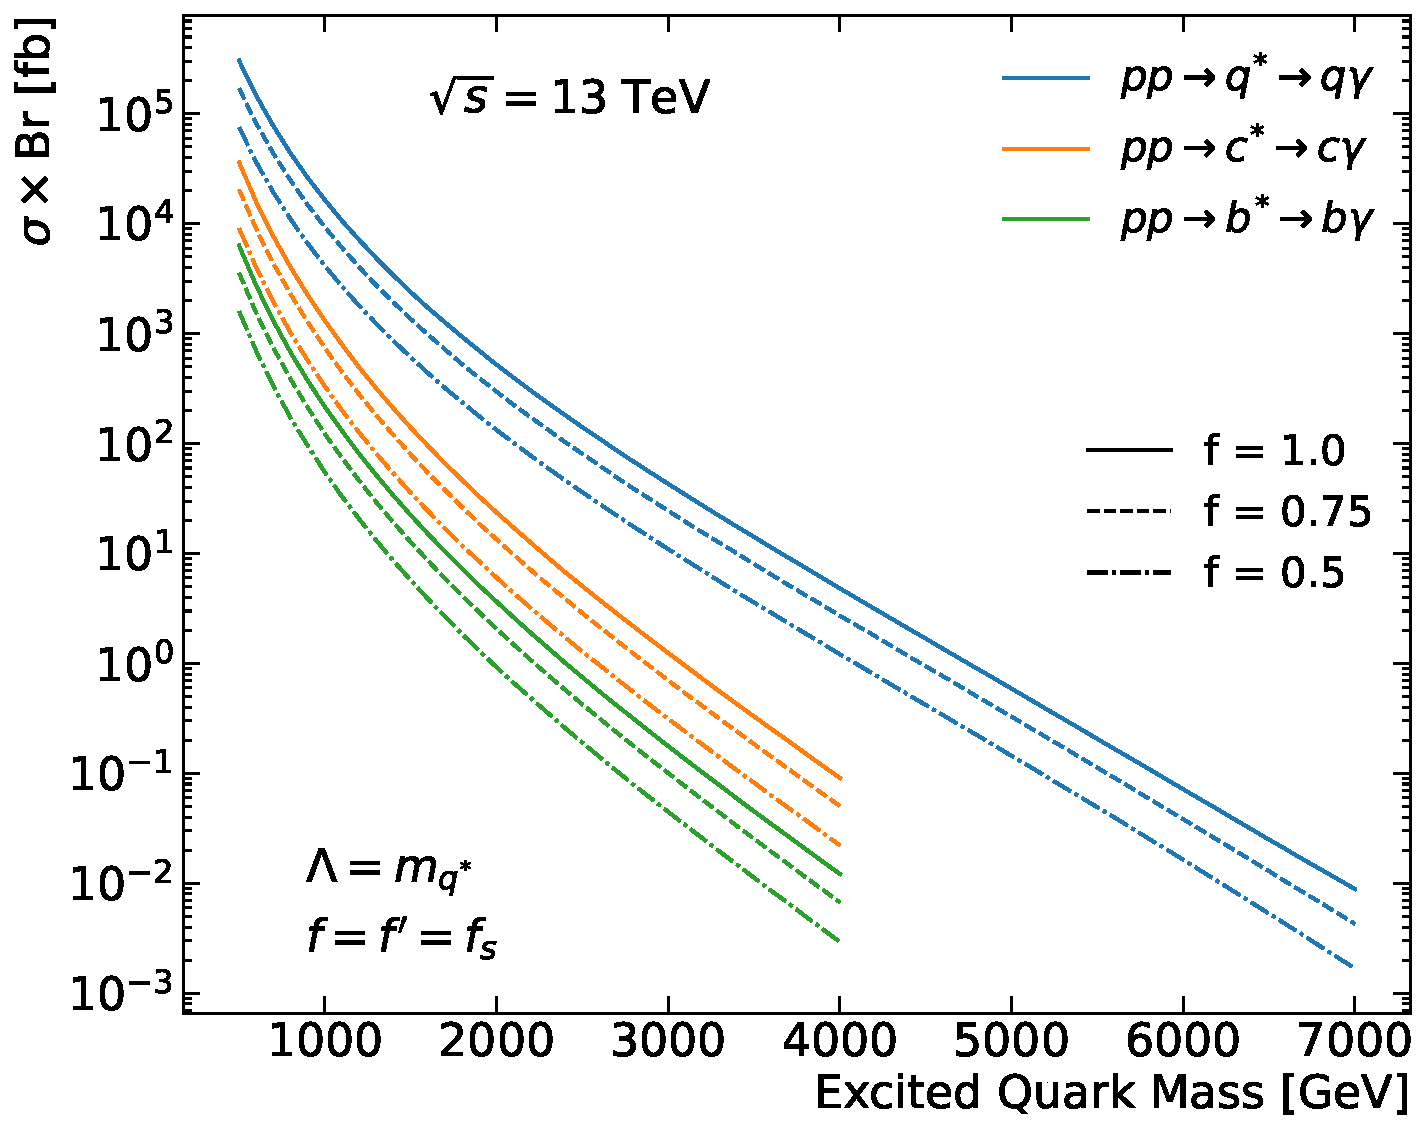
\includegraphics[width=0.6\linewidth]{5_resonances/samples/qstar_xs}
    \caption{Cross-section times branching ratio of the different \ac{EQ} production modes as a function of the \ac{EQ} mass at \(\sqs=13~\tev\). The figure shows the comparison between \qstar (blue), \cstar (orange) and \bstar (green) signals using three different couplings.}
    \label{fig:samples:samples:sig:qstar:xs}
\end{figure}


\subsection{Quantum Black Holes}
\label{subsec:samples:samples:sig:qbh}

\ac{QBH} are predicted to be produced at the \ac{LHC} in \pp collisions, providing a solution to the hierarchy problem through the existence of extra dimensions. 
The production cross section is determined by the gravitational radius which depends on the Planck scale and number of dimensions, formulated as a classical cross section.


Samples of QBH decaying into a photon and a parton are generated with the \ac{QBH} 3.01 software described in \Refn{\cite{QBH}}, and \pythia 8.3 for hadronisation and underlying event. The CTEQ6L1 \ac{PDF1} set has been used together with the standard A14 tuning of the underlying events. The black hole production mass threshold
\(m_{\text{th}}\) is set to be equal to the Planck scale \(m_p\) and the maximum black hole production mass to \(3 m_p\) or the center-of-mass energy \sqs, whichever is less. Two different models are taken into account, depending on the number of extra dimensions \(n\). The ADD model, as discussed in \Sect{\ref{subsec:theory:bsm:qbh}}, considers 6 extra dimensions, leading to a total number 10 space-time dimensions. On the other hand, the RS1 model proposes only one warped extra dimension. Since only the \gammajet final state are of interest for this analysis, the 6 non-thermal black hole states shown in \Sect{\ref{subsec:samples:samples:sig:qbh}} are considered. The cross-sections times branching ratio of the two models are plotted in \Fig{\ref{fig:samples:samples:sig:qbh:xs}}, and the exact numbers shown in \Tab{\ref{tab:samples:samples:sig:qbh:xs}}.


\begin{figure}[ht!]
    \centering
    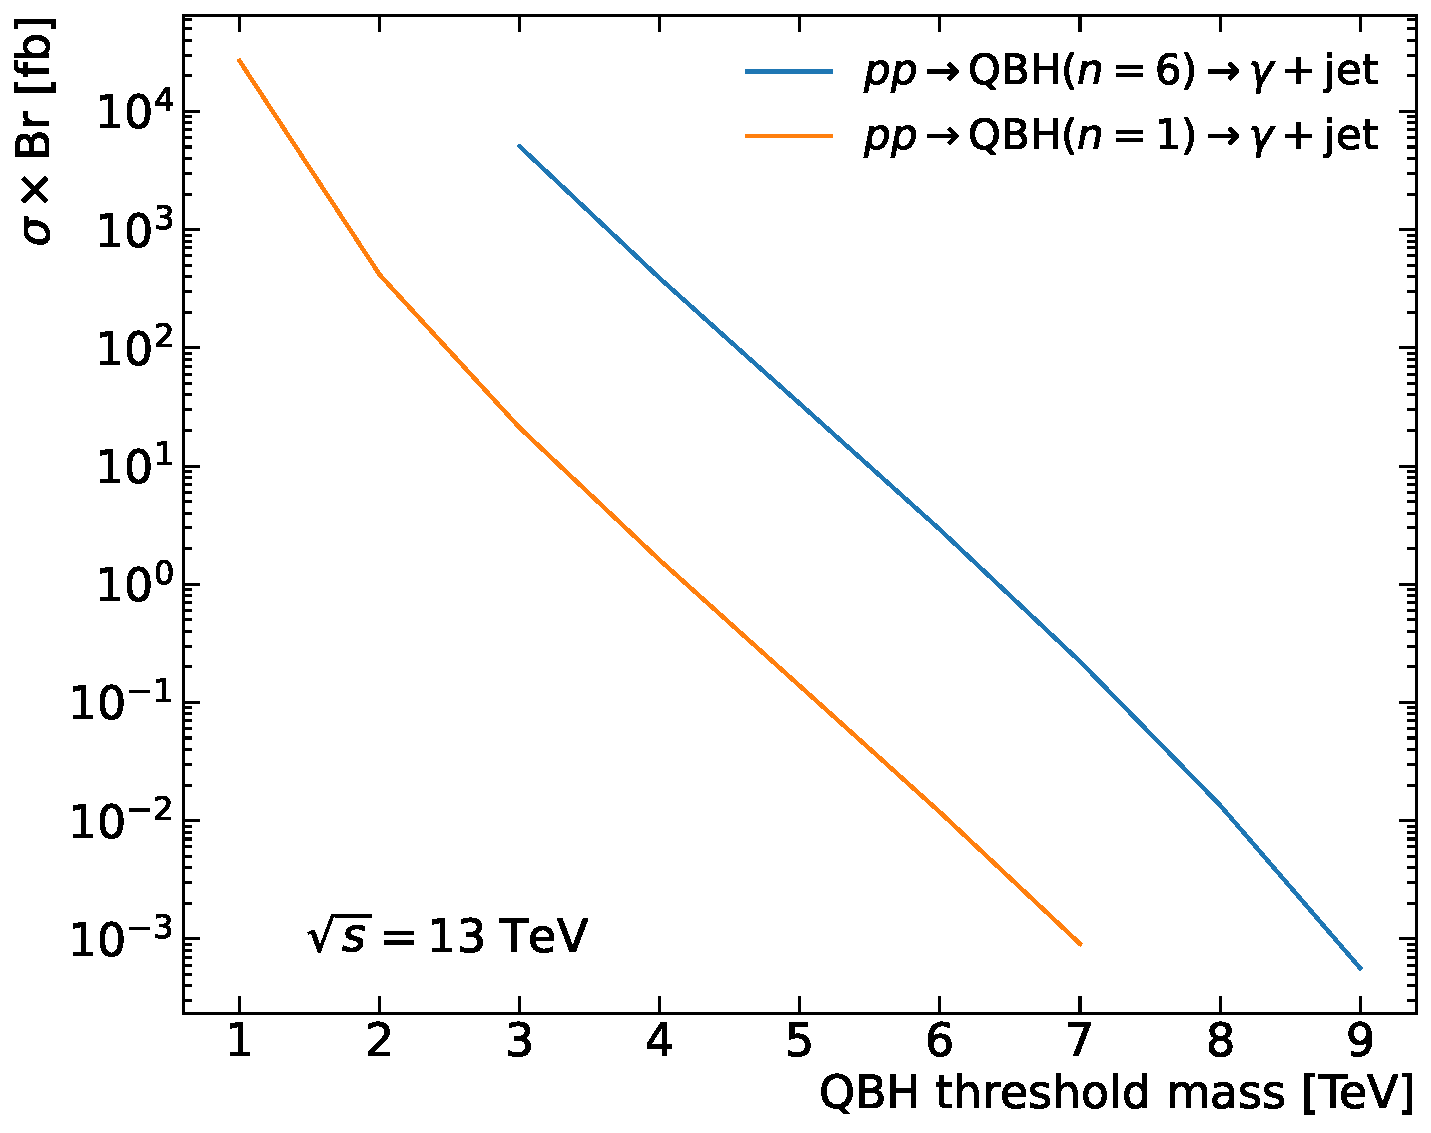
\includegraphics[width=0.6\linewidth]{5_resonances/samples/qbh_xs}
    \caption{Cross-section times branching ratio of the RS1 (orange) and ADD (blue) \ac{QBH} models, for a center-of-mass energy of \(\sqs=13~\tev\).}
    \label{fig:samples:samples:sig:qbh:xs}
\end{figure}


\begin{table}[ht!]
    \caption{Sum of cross section times branching ratio [fb] for the \gammajet final state for the six non-thermal black holes states for each threshold mass \mth.}
    \begin{center}
        \begin{tabular}{ccc}
            \toprule
            \mth [GeV]  & ADD (\(n=6\))         & RS1 (\(n=1\)) \\
            \midrule
            1000        &                       & $2.69\times 10^{+4}$  \\
            2000        &                       & $4.17\times 10^{+2}$  \\
            3000        & $5.07\times 10^{+3}$  & $2.11\times 10^{+1}$  \\
            4000        & $3.88\times 10^{+2}$  & $1.60\times 10^{+0}$  \\
            5000        & $3.37\times 10^{+1}$  & $1.38\times 10^{-1}$  \\
            6000        & $2.90\times 10^{+0}$  & $1.18\times 10^{-2}$  \\
            7000        & $2.22\times 10^{-1}$  & $9.08\times 10^{-4}$  \\
            8000        & $1.35\times 10^{-2}$  &                       \\
            9000        & $5.64\times 10^{-4}$  &                       \\
            \bottomrule
        \end{tabular}
    \end{center}
    \label{tab:samples:samples:sig:qbh:xs}
\end{table}












\section{Backgrounds}
\label{sec:samples:samples:bkg}


In the final state of interest, in which there are at least a photon and a jet, \ac{QCD} prompt photon production is the main \ac{SM} process that cannot be reduced.
To study this particular background contribution, \ac{MC} samples are used.
% To study this particular background contribution, \ac{MC} samples are used, and in this analysis two generators are used.
Moreover, due to mis-identification and mis-reconstruction of jets, there is a considerable fraction of events in which there is at least one jet being mis-identified as a photon. To study this particular contribution, a data-driven approach has been used as described in \Ch{\ref{ch:bkg}}.

% Prompt single-photon production is simulated with the \Sherpa 2.2~\cite{Sherpa2.2} generator. In this set-up, \ac{NLO}-accurate matrix elements for up to two partons, and \ac{LO}-accurate matrix elements for up to four partons are calculated with the Comix~\cite{COMIX} and OpenLoops~\cite{OpenLoops2,OpenLoops1,Collier} libraries. They are matched with the \Sherpa parton shower~\cite{CSDipoleShower} using the \texttt{MEPS@NLO} prescription~\cite{NLOPSMatching,MEPSNLO,MEPSMatching,MEPSLO} with a dynamic merging cut~\cite{SherpaPhotonIsolation} of 20 GeV. Photons are required to be isolated according to a smooth-cone isolation criterion~\cite{FrixioneIsolation}. Samples aare generated using the \NNPDF[3.0nnlo] PDF set~\cite{NNPDF}, along with the dedicated set of tuned parton-shower parameters developed by the Sherpa authors.

Samples of \gammajet with high statistics are generated using the \Pythia 8.186~\cite{Pythia8.1} program. The partonic processes are simulated using \ac{LO} \ac{ME}, with the inclusion of initial- and final-state parton showers, where the parametrisation of the proton structure is given by the \ac{LO} \texttt{NNPDF2.3}~\cite{NNPDF2} \acp{PDF1}.
The hadronisation process is modelled by the Lund string model~\cite{Anderson-1983}, briefly discussed in \Sect{\ref{subsec:theory:mc_simulation:hadronisation}}, and the sample also counts with a simulation of the \ac{UE}.
The event generator parameters are set according to the “A14” tune for \Pythia~\cite{Pythia-A14Tune}.
The \pythia sample, given that it is generated at \ac{LO}, allows for the separation between direct and fragmentation components (see \Sect{\ref{subsec:theory:sm:prompt_photon}}).

The samples are sliced into different regions of \pt to optimise the event generation. Details of each sample, including cross-section and filter efficiencies, are shown in \Tab{\ref{tab:samples:samples:bkg:samples}}.

\begin{table}[ht!]
    \caption{Details of the background \gammajet MC samples}
    \centering
    \resizebox{\textwidth}{!}{
        \begin{tabular}{l c l r r}
            \toprule
            Sample name      &  Generator name                  &   \pt slice [GeV]    & Cross section [pb] &  Filter Eff.  \\
            \midrule
            % \gammajet        &  \sherpa v2.2.2                  &   \([70, 140] \)      & 4526.3            &  1.0          \\
            % \gammajet        &  \sherpa v2.2.2                  &   \([140, 280] \)     & 376.03            &  1.0          \\
            % \gammajet        &  \sherpa v2.2.2                  &   \([280, 500] \)     & 21.864            &  1.0          \\
            % \gammajet        &  \sherpa v2.2.2                  &   \([500, 1000] \)    & 1.4637            &  1.0          \\
            % \gammajet        &  \sherpa v2.2.2                  &   \([1000, \infty]\)  & 0.029854          &  1.0          \\
            % \midrule
            \gammajet direct &  \Pythia 8.244.3+\EvtGen v.1.7.0 &  \([70, 140]\)        & 28396.0           &  7.2863E-02   \\
            \gammajet direct &  \Pythia 8.244.3+\EvtGen v.1.7.0 &  \([140, 280]\)       & 2625.5            &  7.0598E-02   \\
            \gammajet direct &  \Pythia 8.244.3+\EvtGen v.1.7.0 &  \([280, 500]\)       & 198.39            &  6.0369E-02   \\
            \gammajet direct &  \Pythia 8.244.3+\EvtGen v.1.7.0 &  \([500, 800]\)       & 18.846            &  4.4596E-02   \\
            \gammajet direct &  \Pythia 8.244.3+\EvtGen v.1.7.0 &  \([800, 1000]\)      & 2.3312            &  2.4130E-02   \\
            \gammajet direct &  \Pythia 8.244.3+\EvtGen v.1.7.0 &  \([1000, 1500]\)     & 0.79945           &  2.3667E-02   \\
            \gammajet direct &  \Pythia 8.244.3+\EvtGen v.1.7.0 &  \([1500, 2000]\)     & 0.055512          &  1.9632E-02   \\
            \gammajet direct &  \Pythia 8.244.3+\EvtGen v.1.7.0 &  \([2000, 2500]\)     & 0.0052361         &  1.6644E-02   \\
            \gammajet direct &  \Pythia 8.244.3+\EvtGen v.1.7.0 &  \([2500, 3000]\)     & 0.00052733        &  1.4446E-02   \\
            \gammajet direct &  \Pythia 8.244.3+\EvtGen v.1.7.0 &  \([3000, \infty]\)   & 4.8856e-05        &  1.4371E-02   \\
            \gammajet frag   &  \Pythia 8.244.3+\EvtGen v.1.7.0 &  \([70, 140]\)        & 106180000.0       &  1.9271E-05   \\
            \gammajet frag   &  \Pythia 8.244.3+\EvtGen v.1.7.0 &  \([140, 280]\)       & 6702000.0         &  2.0959E-05   \\
            \gammajet frag   &  \Pythia 8.244.3+\EvtGen v.1.7.0 &  \([280, 500]\)       & 344070.0          &  2.0507E-05   \\
            \gammajet frag   &  \Pythia 8.244.3+\EvtGen v.1.7.0 &  \([500, 800]\)       & 23711.0           &  1.6991E-05   \\
            \gammajet frag   &  \Pythia 8.244.3+\EvtGen v.1.7.0 &  \([800, 1000]\)      & 2284.6            &  1.0123E-05   \\
            \gammajet frag   &  \Pythia 8.244.3+\EvtGen v.1.7.0 &  \([1000, 1500]\)     & 701.22            &  1.0074E-05   \\
            \gammajet frag   &  \Pythia 8.244.3+\EvtGen v.1.7.0 &  \([1500, 2000]\)     & 70.086            &  5.0238E-06   \\
            \gammajet frag   &  \Pythia 8.244.3+\EvtGen v.1.7.0 &  \([2000, \infty]\)   & 11.548            &  2.4464E-06   \\
            \bottomrule
        \end{tabular}
    }
    \label{tab:samples:samples:bkg:samples}
\end{table}

As discussed in \Sect{\ref{sec:strategy:strategy}}, the background in the final data samples is estimated in a data-driven way using different functional forms. \ac{MC} background samples, nevertheless, are used to filter and rank the most optimal functions.